\chapter{Methodology}
We describe the baseline and attention\textendash augmented architectures, formalize CBAM, and motivate design choices (placement, reduction ratio, kernel size). We also outline training and evaluation protocols to ensure a fair comparison and reproducibility.
\section{Baselines and Architecture}
\textbf{EfficientNet Baseline:} ImageNet\textendash pretrained EfficientNetB0 (optionally B3) with a light classification head: BN $\rightarrow$ Conv1x1 (192) $\rightarrow$ GAP $\rightarrow$ Dropout(0.4) $\rightarrow$ Dense(192, ReLU) $\rightarrow$ Dropout(0.4) $\rightarrow$ Softmax.

\textbf{EfficientNet + CBAM:} Same backbone and head, with a CBAM block applied on the convolutional feature map to apply channel and spatial attention.

% 1) Start with attention concept + base attention figure
\begin{figure}[t]
  \centering
  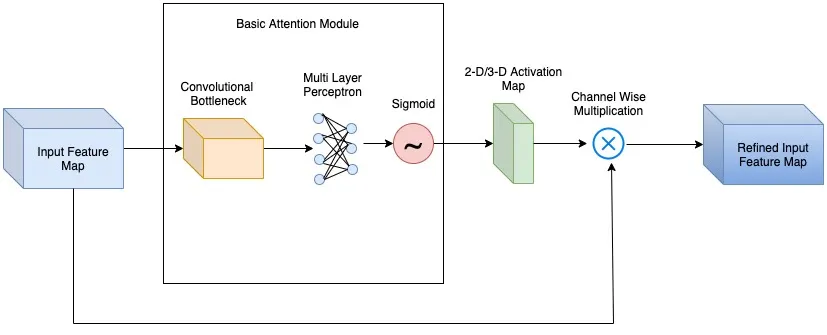
\includegraphics[width=0.9\textwidth]{../new_work/figures/about-cbam/base-attention-model.png}
  \caption{Base attention idea: an attention map refines intermediate feature maps to emphasize informative content and suppress background, improving downstream classification. Adapted for context from primers \cite{cbamMedium}.}
  \label{fig:base_attention}
\end{figure}

\subsection{CBAM Details}
CBAM introduces lightweight attention along two axes \cite{woo2018cbam,cbamMedium,cbamDO}:
\begin{itemize}
  \item \textbf{Channel attention (what):} statistics are pooled via both global average and max pooling and passed through a shared MLP to produce per\textendash channel weights in $(0,1)$ via $\sigma$. This emphasizes informative feature channels while suppressing less useful ones.
  \item \textbf{Spatial attention (where):} the feature map is aggregated across channels using average and max projections and filtered by a $7\times7$ convolution to produce a spatial mask highlighting salient regions.
  \item \textbf{Sequential composition:} channel attention is applied first, followed by spatial attention, i.e., $F' = M_s(M_c(F)\odot F)\odot F$. This ordering empirically outperforms the reverse or parallel setups.
  \item \textbf{Design contrasts to BAM:} unlike BAM that uses dilated convolutions to enlarge receptive fields, CBAM relies on a larger kernel ($7\times7$) with standard dilation and augments average pooling with max pooling, improving saliency capture \cite{cbamMedium}.
\end{itemize}

\begin{figure}[t]
  \centering
  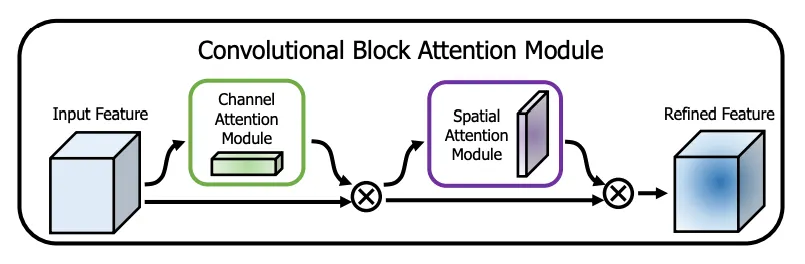
\includegraphics[width=0.95\textwidth]{../new_work/figures/about-cbam/cbam-architecture.png}
  \caption{CBAM module: sequential channel and spatial attention with shared MLP for channel pooling (Avg/Max) and a $7\times7$ conv for spatial pooling. See \cite{woo2018cbam,cbamMedium,cbamDO}.}
  \label{fig:cbam_module}
\end{figure}

\begin{figure}[t]
  \centering
  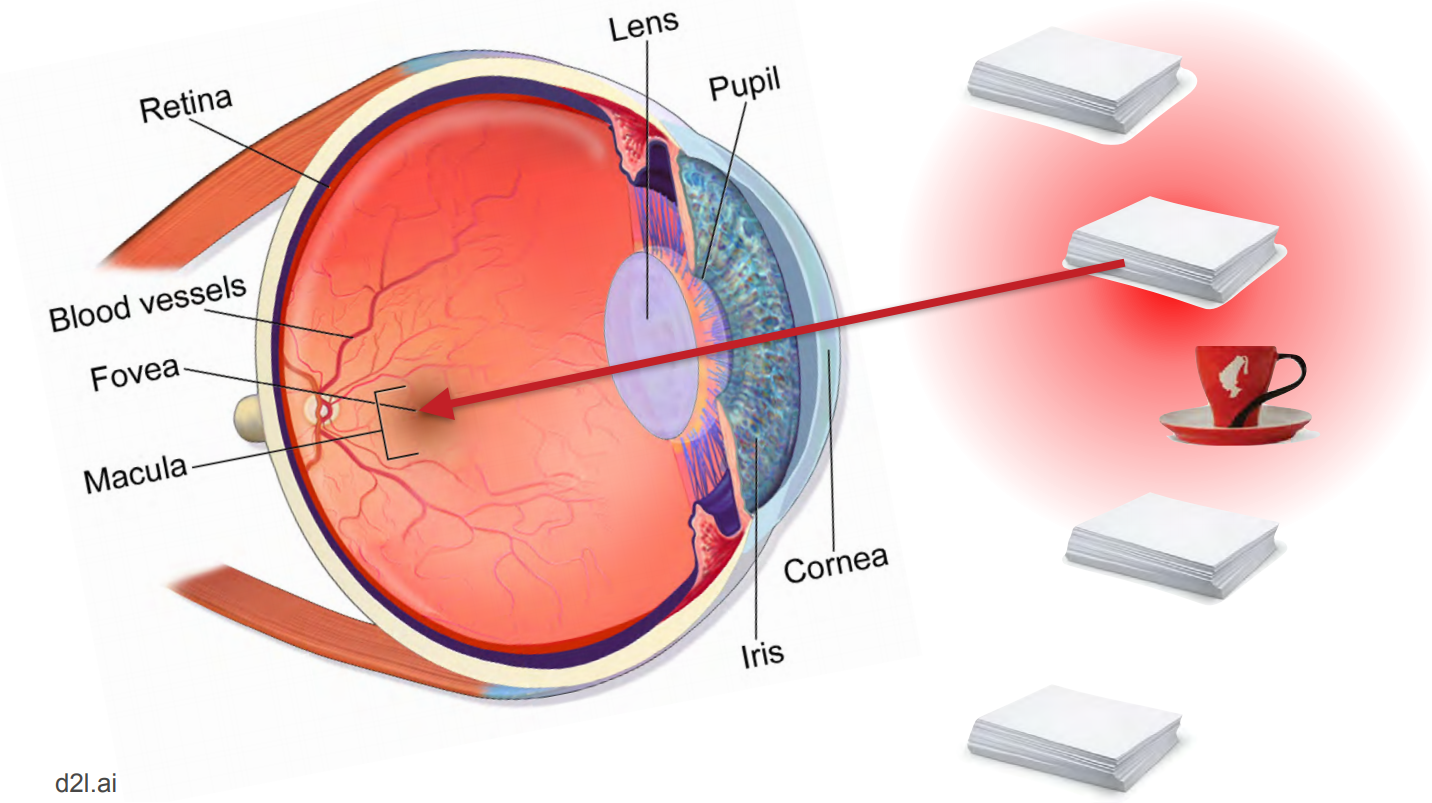
\includegraphics[width=0.92\textwidth]{../new_work/websites/Attention Mechanisms in Computer Vision_ CBAM _ DigitalOcean_files/image-1.png}
  \caption{Channel and spatial attention paths in CBAM (DigitalOcean \cite{cbamDO}). The channel branch uses global average and max pooling with a shared MLP; the spatial branch aggregates across channels and uses a $7\times7$ convolution to produce a saliency mask.}
  \label{fig:cbam_do_paths}
\end{figure}

\subsection{Theory of Attention: From Tokens to Feature Maps}
Let $Q\in\mathbb{R}^{n\times d}$, $K\in\mathbb{R}^{m\times d}$, and $V\in\mathbb{R}^{m\times d\_v}$ denote queries, keys, and values for a set of $n$ queries and $m$ key\textendash value pairs. Scaled dot\textendash product attention \cite{vaswani2017attention} computes
\[ \mathrm{Attn}(Q,K,V) = \mathrm{softmax}\!\Big( \tfrac{QK^\top}{\sqrt{d}} \Big) V. \]
Multi\textendash head attention projects $(Q,K,V)$ into $h$ subspaces and concatenates results to increase representational capacity at similar cost via parallel heads.

In token models (e.g., ViT \cite{dosovitskiy2021vit}, DeiT \cite{touvron2021deit}), $Q,K,V$ are derived from flattened image patches. In CNNs, the spatial grid and channels already encode strong inductive biases (locality, translation), so lighter attentional reweighting often suffices. CBAM acts directly on the convolutional feature map $F\in\mathbb{R}^{H\times W\times C}$, learning \/what\/ (channels) and \/where\/ (spatial) to emphasize without computing global token\textendash token affinities.

\subsection{CBAM Formulation with Equations}
Given $F\in\mathbb{R}^{H\times W\times C}$, CBAM computes channel attention $M\_c\in(0,1)^C$ by pooling along spatial dimensions with both average and max pooling, then passing through a shared MLP with reduction ratio $r$:
\[ M\_c(F) = \sigma\big( \mathrm{MLP}(\mathrm{AvgPool}(F)) + \mathrm{MLP}(\mathrm{MaxPool}(F)) \big), \quad \mathrm{MLP}: \mathbb{R}^{C} \to \mathbb{R}^{C/r} \to \mathbb{R}^{C}. \]
Channel\textendash refined features: $F' = M\_c(F) \odot F$. Spatial attention $M\_s\in(0,1)^{H\times W}$ is computed by concatenating channel\textendash wise average and max projections, then filtering with a $k\times k$ convolution (typically $k{=}7$):
\[ M\_s(F') = \sigma\Big( \mathrm{Conv}_{k\times k}\big([\mathrm{AvgProj}(F');\,\mathrm{MaxProj}(F')]\big) \Big). \]
The output is $F'' = M\_s(F') \odot F'$. The sequential order (channel then spatial) empirically yields stronger gains than the reverse or parallel variants \cite{woo2018cbam}.

\paragraph{Design Choices.}
\textbf{Reduction ratio $r$.} Smaller $r$ increases MLP capacity; we set $r{=}16$ for a good accuracy\textendash cost balance. \textbf{Kernel size $k$.} A larger spatial kernel (e.g., $7$) expands the effective receptive field of attention without heavy dilation \cite{cbamMedium}. \textbf{Pooling types.} Using both average and max pooling stabilizes gradients and captures complementary statistics.

\paragraph{Complexity and Overhead.}
CBAM adds $\mathcal{O}(C^2/r)$ parameters in the channel MLP and one shallow $k\times k$ spatial convolution. For EfficientNetB0 features ($C\approx 1280$ at the last block), $r{=}16$ keeps overhead small relative to the backbone while delivering robust gains. Unlike token attention with quadratic cost in sequence length, CBAM's cost is linear in spatial size and dominated by the small MLP and single convolution.

\subsection{Placement in EfficientNet and Integration Strategy}
We insert CBAM immediately after the final convolutional block outputs and before the classification head (Figure~\ref{fig:cbam_arch}). Placing attention late focuses the classifier on semantically rich channels and locations while preserving EfficientNet's early\textendash stage inductive biases and pretraining benefits. We then apply a lightweight head: BN $\rightarrow$ Conv1x1 (192) $\rightarrow$ GAP $\rightarrow$ Dropout $\rightarrow$ Dense(192, ReLU) $\rightarrow$ Dropout $\rightarrow$ Softmax.

\paragraph{Why not earlier or multiple CBAMs?}
Early layers represent low\textendash level edges and textures where heavy reweighting may reduce transferability from ImageNet. Multiple CBAMs increase cost and may require careful tuning of $r$ and $k$. A single late CBAM provided clear value\textendash add within our memory budget.

\subsection{Training Stability and Practical Notes}
We enable mixed precision (float16 compute, float32 logits) to save memory, add a one\textendash time warm\textendash up forward pass to stabilize cuDNN timers, and row\textendash normalize confusion matrices to percentages for clearer per\textendash class error profiles. Class weighting mitigates the Hypertension minority. We keep the final Dense output in float32 to avoid numerical underflow in cross\textendash entropy.

Mixed precision is a critical optimization for modern GPUs. By performing high\textendash FLOPS operations (convolutions, GEMMs) in float16, we approximately halve activation and gradient memory footprint, enabling either larger models or larger batch sizes. Larger batches yield more stable gradient estimates per step, often accelerating and stabilizing convergence. Hardware (e.g., NVIDIA Tensor Cores) further accelerates float16 matrix ops, commonly yielding 2\textendash 3x wall\textendash clock speedups.

Float16's limited dynamic range introduces risks of underflow/overflow. We therefore use dynamic loss scaling to keep gradients within representable ranges, scaling down before the optimizer step. We also retain the final output layer and loss computation in float32: the softmax\textendash cross\textendash entropy pathway is numerically sensitive, and low\textendash magnitude logits in float16 can underflow toward negative infinity, producing unstable log probabilities. Keeping the head in float32 preserves a reliable loss signal.

The cuDNN warm\textendash up pass avoids anomalously slow first iterations during auto\textendash tuning. cuDNN selects convolution algorithms on the first pass based on input/filter shapes; performing one untimed forward/backward warms these selections so subsequent iterations reflect steady\textendash state throughput.

Finally, row\textendash normalizing the confusion matrix is essential under imbalance. Raw counts are dominated by majority classes and hard to interpret. Normalizing each row by its sum expresses per\textendash class recall distributions: row $i$ shows how true class $i$ is distributed across predicted classes. This immediately surfaces actionable patterns (e.g., a fraction of Hypertension mislabeled as Normal) that raw counts obscure.

\subsection{Summary of Attention vs CBAM for Fundus Images}
Token self\textendash attention (e.g., ViT/DeiT) excels with large data and aggressive augmentation but is data\textendash hungry due to weak inductive bias. CNNs embed strong priors (locality, translation equivariance) that perform well on modest datasets, learning robust features with fewer samples. For ODIR\textendash 5K scale, a hybrid that augments a strong CNN (EfficientNet) with lightweight attention (SE \cite{hu2018squeeze}, ECA \cite{wang2020eca}, BAM \cite{park2018bam}, CBAM \cite{woo2018cbam}) is typically more parameter\textendash efficient and stable.

ViTs treat images as patch sequences and learn spatial relations primarily via global self\textendash attention. Without large\textendash scale pretraining, ViTs can overfit small medical datasets or learn brittle patch statistics. In contrast, EfficientNet provides a well\textendash calibrated feature hierarchy. Adding CBAM refines these features with minimal overhead: channel attention learns \emph{what} to emphasize by re\textendash weighting discriminative channels (e.g., vasculature patterns), while spatial attention learns \emph{where} to focus by highlighting salient retinal regions (disc, macula). This combination preserves CNN inductive bias while granting explicit saliency control, which our experiments show yields consistent gains over the baseline.

% 3) Finally, our EfficientNet + CBAM integration
\begin{figure}[t]
  \centering
  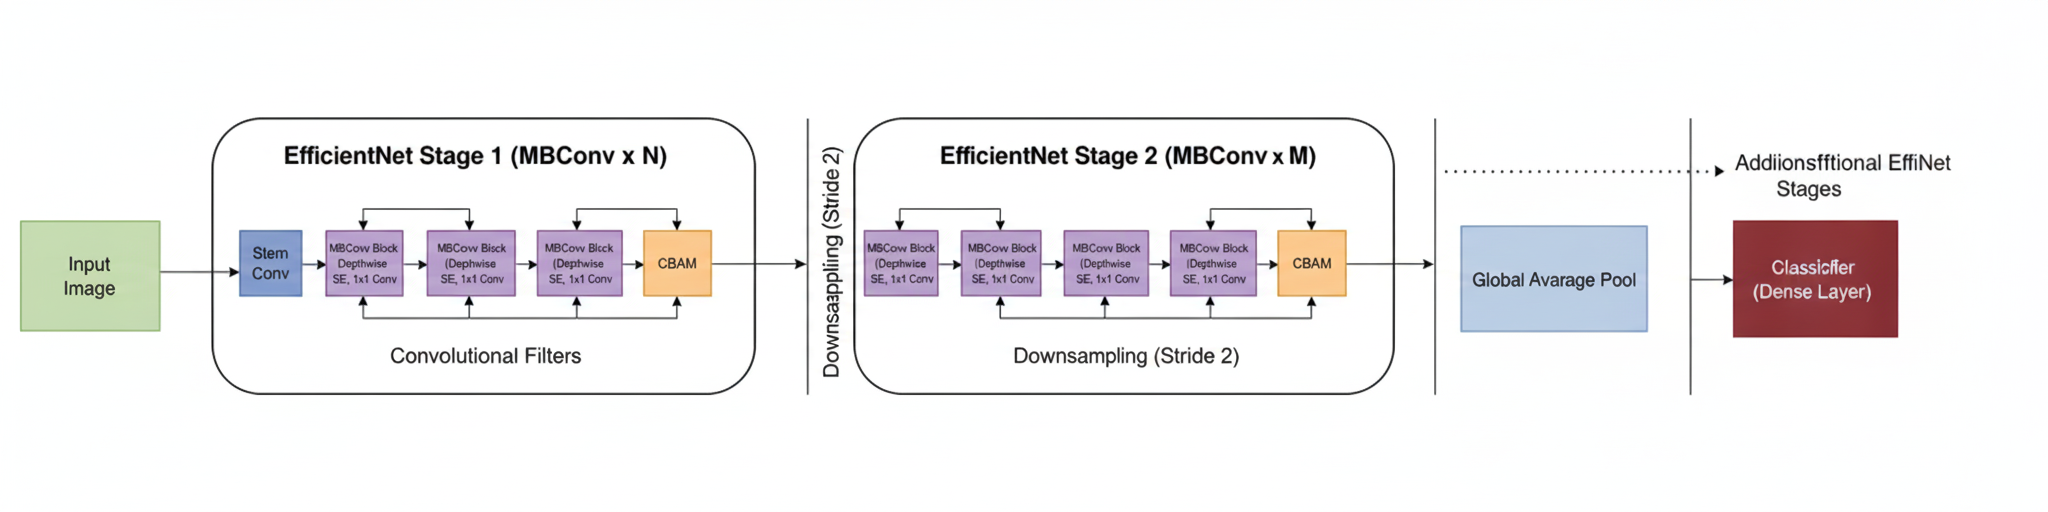
\includegraphics[width=0.9\textwidth]{../new_work/figures/about-cbam/EfficientNet-placement-with-CBAM-architecture.png}
  \caption{Our architecture: EfficientNet backbone with a CBAM attention block over feature maps, followed by a lightweight classification head.}
  \label{fig:cbam_arch}
\end{figure}

\section{Training}
\textbf{Optimizer and Schedule.} We use Adam with learning rate $3\times 10^{-4}$ and batch size 16, along with a one\textendash time warm\textendash up pass. Callbacks include ModelCheckpoint (monitoring validation accuracy), ReduceLROnPlateau, and EarlyStopping with best\textendash weight restore. Mixed precision is enabled for memory efficiency and throughput.

\textbf{ModelCheckpoint (best val acc).} At epoch end we save weights achieving a new best validation accuracy, ensuring final evaluation uses the best\textendash generalizing checkpoint rather than the last epoch.

\textbf{ReduceLROnPlateau.} If validation accuracy plateaus for several epochs, we reduce the learning rate (e.g., by 10x) to allow finer convergence in a narrower basin of the loss landscape.

\textbf{EarlyStopping.} If no improvement occurs for a longer patience window, we stop training and restore the best weights, preventing overfitting and saving compute.

\paragraph{Loss and Metrics.} We optimize categorical cross\textendash entropy over 5 classes (G, C, A, H, M), acknowledging ODIR\textendash 5K's underlying multi\textendash label nature as a pragmatic simplification. We report accuracy; macro and weighted F1; ROC\textendash AUC (macro, one\textendash vs\textendash rest); and PR\textendash AUC (macro). Let $\hat{y}\_{i,c}$ be the predicted probability for class $c$ and $y\_{i,c}\in\{0,1\}$. The loss is
\[ \mathcal{L} = -\sum\_{i}\sum\_{c} y\_{i,c}\log\big(\hat{y}\_{i,c}\big). \]
Macro F1 averages per\textendash class F1 without weighting, emphasizing minority classes; weighted F1 weights by class support. ROC\textendash AUC (OvR, macro) evaluates discrimination at all thresholds; PR\textendash AUC is especially informative under class imbalance where true negatives are abundant.

\section{Evaluation}
We report accuracy, macro/weighted F1, ROC\textendash AUC (macro one\textendash vs\textendash rest), PR\textendash AUC (macro), and confusion matrices. Curves (training/validation for accuracy, loss, ROC\textendash AUC, PR\textendash AUC) and per\textendash class ROC/PR curves are exported.

\paragraph{CBAM Primer.} CBAM sequentially applies channel attention and spatial attention \cite{woo2018cbam}, reweighting feature channels (\emph{what}) and spatial locations (\emph{where}). We reference succinct primers \cite{cbamMedium,cbamDO} for intuition and module design.

\paragraph{Implementation Notes.} We integrate CBAM after the final EfficientNet convolutional block and before the classification head (Figure~\ref{fig:cbam_arch}). Channel attention uses a shared MLP with reduction ratio $r=16$; spatial attention uses a $7\times7$ convolution on concatenated average and max projections, following \cite{woo2018cbam,cbamDO}. We row\textendash normalize confusion matrices to percentages to reflect per\textendash class error structure.

